%%%%%%%%%%%%%%%%%%%%%%%%%%%%%%%%%%%%%%%%%%%%%%%%%%%%%%%%%%%%%%%%%%%%%%
% UMB-CS110-2015S: Introduction to Computing
% Copyright 2015 Pejman Ghorbanzade <pejman@ghorbanzade.com>
% Creative Commons Attribution-ShareAlike 4.0 International License
% More info: https://github.com/ghorbanzade/UMB-CS110-2015S
%%%%%%%%%%%%%%%%%%%%%%%%%%%%%%%%%%%%%%%%%%%%%%%%%%%%%%%%%%%%%%%%%%%%%%

\def \topDirectory {../..}
\def \texDirectory {\topDirectory/src/main/tex}

\documentclass[10pt, compress]{beamer}

\usepackage{\texDirectory/template/style/directives}
%%%%%%%%%%%%%%%%%%%%%%%%%%%%%%%%%%%%%%%%%%%%%%%%%%%%%%%%%%%%%%%%%%%%%%%%%%%%%%
% CS110: Introduction to Computing
% Copyright 2015 Pejman Ghorbanzade <mail@ghorbanzade.com>
% Creative Commons Attribution-ShareAlike 4.0 International License
% https://github.com/ghorbanzade/UMB-CS110-2015S/blob/master/LICENSE
%%%%%%%%%%%%%%%%%%%%%%%%%%%%%%%%%%%%%%%%%%%%%%%%%%%%%%%%%%%%%%%%%%%%%%%%%%%%%%

\course{id}{CS110}
\course{name}{Introduction to Computing}
\course{venue}{Tue/Thu, 5:30 PM - 6:45 PM}
\course{semester}{Spring 2015}
\course{department}{Department of Computer Science}
\course{university}{University of Massachusetts Boston}

\instructor{name}{Pejman Ghorbanzade}
\instructor{title}{}
\instructor{position}{Student Instructor}
\instructor{email}{pejman@cs.umb.edu}
\instructor{phone}{617-287-6419}
\instructor{office}{S-3-124B}
\instructor{office-hours}{Tue/Thu 19:00-20:30}
\instructor{address}{University of Massachusetts Boston, 100 Morrissey Blvd., Boston, MA}

\usepackage{\texDirectory/template/style/beamerthemeUmassLecture}
\doc{number}{17}
%\setbeamertemplate{footline}[text line]{}

\begin{document}
\prepareCover

\section{Course Administration}

\begin{frame}[fragile]
\frametitle{Course Administration}
Deadline for Assignment 5 extended to May 3, 2015 at 11:59 PM.
\end{frame}

\begin{frame}[fragile]
	\frametitle{Overview}
	\begin{itemize}
		\item[] Sorting Algorithms
		\begin{itemize}
			\item[] Introduction
			\item[] Bogo Sort
			\item[] Selection Sort
			\item[] Insertion Sort
			\item[] Bubble Sort
		\end{itemize}
	\end{itemize}
\end{frame}

\plain{}{Sorting Algorithms}

\section{Introduction}

\begin{frame}[fragile]
	\frametitle{Sorting Algorithms}
	\begin{figure}
		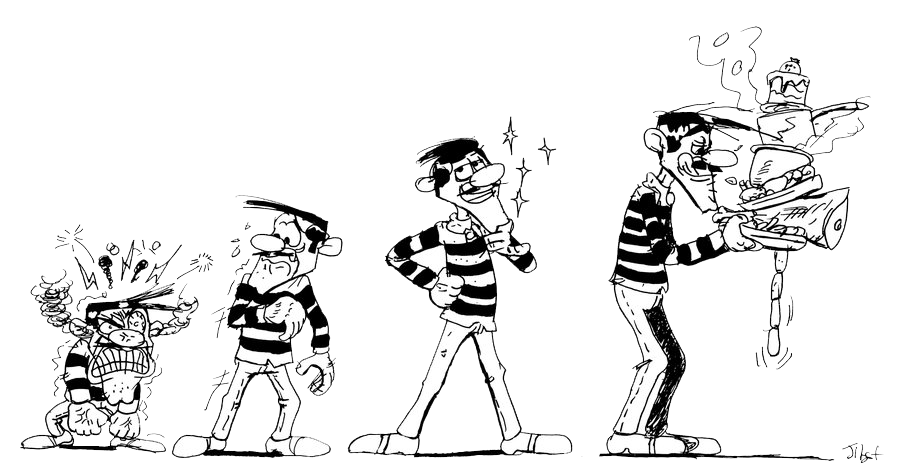
\includegraphics[width=\textwidth]{\texDirectory/template/images/daltons.png}
	\end{figure}
\end{frame}

\begin{frame}[fragile]
	\frametitle{Sorting Algorithms}
	\begin{block}{Definition}
		Sorting is the process of rearranging a sequence of objects so as to put them in some logical order.
	\end{block}
\end{frame}

\begin{frame}[fragile]
	\frametitle{Sorting Algorithms}
	\begin{block}{Motivation}
		\begin{itemize}
			\item[] Organization of Data
			\item[] Accessibility of Data
			\item[] Efficient Data Processing
			\item[] Efficient Data Management
		\end{itemize}
	\end{block}
\end{frame}

\begin{frame}[fragile]
	\frametitle{Sorting Algorithms}
	\begin{block}{Objective}
		Write a program \texttt{StudentSort.java} to sort 10 students of class \texttt{Student.java} with random heights between 150 cm and 190 cm based on their heights.
	\end{block}
\end{frame}

\begin{frame}[fragile]
	\frametitle{Sorting Algorithms}
	\begin{block}{\texttt{Student.java} (v1.0)}
		\begin{minted}[fontsize=\small,linenos,firstnumber=1]{java}
public class Student {
	private double height;
	public double getHeight() {
		return height;
	}
	public Student() {
		this.height = Math.round(150 + Math.random()*40);
	}
}
		\end{minted}
	\end{block}
\end{frame}

\begin{frame}[fragile]
	\frametitle{Sorting Algorithms}
	\begin{block}{\texttt{StudentSort.java} (v1.0) (Page 1)}
		\begin{minted}[fontsize=\small,linenos,firstnumber=1]{java}
public class StudentsSort {
	public static void main(String[] args) {
		Student[] students = new Student[10];
		// Initialize array with students
		init(students);
		show(students);
		// Shuffle students in row
		shuffle(students);
		show(students);
		// Sort students
		sort(students);
		show(students);
	}
		\end{minted}
	\end{block}
\end{frame}

\begin{frame}[fragile]
	\frametitle{Sorting Algorithms}
	\begin{block}{\texttt{StudentSort.java} (v1.0) (Page 2)}
		\begin{minted}[fontsize=\small,linenos,firstnumber=14]{java}
	public static void show(Student[] array) {
		for (int i = 0; i < array.length; i++)
			System.out.printf("%d, ", (int) array[i].getHeight());
		System.out.println();
	}
	public static void init(Student[] array) {
		for (int i = 0; i < array.length; i++)
			array[i] = new Student();
	}
	public static void exchange(Student[] array, int i, int j) {
		Student temp = array[i];
		array[i] = array[j];
		array[j] = temp;
	}
		\end{minted}
	\end{block}
\end{frame}

\begin{frame}[fragile]
	\frametitle{Sorting Algorithms}
	\begin{block}{\texttt{StudentSort.java} (v1.0) (Page 3)}
		\begin{minted}[fontsize=\small,linenos,firstnumber=28]{java}
	public static void shuffle(Student[] array) {
		for (int i = 0; i < array.length; i++) {
			int j = i + (int) (Math.random()*(array.length-i));
			exchange(array, i, j);
		}
	}
	public static boolean isSorted(Student[] array) {
		for (int i = 0; i < array.length-1; i++)
			if (array[i].getHeight() > array[i+1].getHeight())
				return false;
		return true;
	}
	public static void sort(Student[] array) {
		// how to sort!?
	}
}
		\end{minted}
	\end{block}
\end{frame}

\begin{frame}[fragile]
	\frametitle{Sorting Algorithms}
	\begin{block}{How to sort!?}
	There are many different ways to sort elements of an array.
		\begin{figure}
			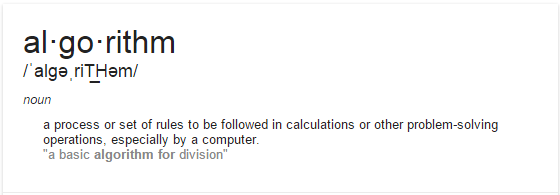
\includegraphics[width=\textwidth]{\texDirectory/template/images/algorithm.png}
		\end{figure}
	\end{block}
\end{frame}

\begin{frame}[fragile]
	\frametitle{Sorting Algorithms}
	\begin{block}{How to sort}
	There are many different algorithms to sort elements of an array.
	\begin{columns}
		\begin{column}{0.3\textwidth}
			\begin{itemize}
				\item[] Insertion Sort
				\item[] Selection Sort
				\item[] Bubble Sort
				\item[] Merge Sort
				\item[] Quick Sort
				\item[] Heap Sort
			\end{itemize}
		\end{column}
		\begin{column}{0.3\textwidth}
			\begin{itemize}
				\item[] Shell Sort
				\item[] Radix Sort
				\item[] Cycle Sort
					\item[] Bucket Sort
 				\item[] Counting Sort
 				\item[] Spaghetti Sort
			\end{itemize}
		\end{column}
		\begin{column}{0.4\textwidth}
			\begin{itemize}
				\item[] Tim Sort
				\item[] Comb Sort
				\item[] Smooth Sort
				\item[] Odd-Even Sort
				\item[] Cocktail Shaker Sort
				\item[] Batcher's Bitonic Sort
			\end{itemize}
		\end{column}
	\end{columns}
	\end{block}
\end{frame}

\begin{frame}[fragile]
	\frametitle{Sorting Algorithms}
	\begin{block}{How to Sort}
	What is the best algorithm to sort an array?
		\begin{itemize}
			\item[] Runtime complexity of the algorithm
			\item[] Memory requirements of the algorithm
			\item[] Stability of the algorithm
			\item[] In-placement of the algorithm
			\item[] Randomness of the array to be sorted
			\item[] Size of the array to be sorted
			\item[] Platform on which sorting algorithm should be implemented
		\end{itemize}
	\end{block}
\end{frame}

\section{Bogo Sort}

\begin{frame}[fragile]
	\frametitle{Sorting Algorithms}
	\begin{block}{\texttt{StudentSort.java} (v2.0) (Page 3)}
		\begin{minted}[fontsize=\small,linenos,firstnumber=40]{java}
	// Bogo Sort
	public static void sort(Student[] array) {
		while (!isSorted(array))
			shuffle(array);
	}
		\end{minted}
	\end{block}
\end{frame}

\begin{frame}[fragile]
	\frametitle{Sorting Algorithms}
	\begin{block}{Bogo Sort}
		Bogo Sort (AKA. Stupid Sort) is the most inefficient algorithm to sort an array that keeps shuffling the array as long as it's not sorted.
	\end{block}
\end{frame}

\begin{frame}[fragile]
	\frametitle{Sorting Algorithms}
	\begin{block}{Analysis of Bogosort}
		\begin{itemize}
			\item[] Expected number of comparisons:\hfill $(e-1)n!$
			\item[] Expected number of swaps:\hfill $(n-1)n!$
			\item[] Best-case runtime:\hfill $\mathcal{O}(n)$
			\item[] Average-case runtime:\hfill $\mathcal{O}((n+1)!)$
			\item[] Worst case runtime:\hfill $\infty$
		\end{itemize}
	\end{block}
\end{frame}

\section{Selection Sort}

\begin{frame}[fragile]
	\frametitle{Sorting Algorithms}
	\begin{block}{\texttt{StudentSort.java} (v3.0) (Page 3)}
		\begin{minted}[fontsize=\small,linenos,firstnumber=40]{java}
	// Selection Sort
	public static void sort(Student[] array) {
		for (int i = 0; i < array.length; i++) {
			int min = i;
			for (int j = i+1; j < array.length; j++)
				if (array[j].getHeight() < array[min].getHeight())
					min = j;
			exchange(array, i, min);
		}
	}
		\end{minted}
	\end{block}
\end{frame}

\begin{frame}[fragile]
	\frametitle{Sorting Algorithms}
	\begin{block}{Selection Sort}
		Selection Sort is a simple, in-place yet expensive and unstable sorting algorithm.

		Selection Sort divides the array into two sorted and unsorted parts, placing element with least value of the unsorted part in rightmost side of the sorted part until the unsorted part is empty.
	\end{block}
\end{frame}

\begin{frame}[fragile]
	\frametitle{Sorting Algorithms}
	\begin{block}{Analysis of Selection Sort}
		\begin{itemize}
			\item[] Expected number of comparisons:\hfill $\mathcal{O}(n^2)$
			\item[] Expected number of swaps:\hfill $\mathcal{O}(n)$
			\item[] Best-case runtime:\hfill $\mathcal{O}(n^2)$
			\item[] Average-case runtime:\hfill $\mathcal{O}(n^2)$
			\item[] Worst case runtime:\hfill $\mathcal{O}(n^2)$
		\end{itemize}
	\end{block}
\end{frame}

\section{Insertion Sort}

\begin{frame}[fragile]
	\frametitle{Sorting Algorithms}
	\begin{block}{\texttt{StudentSort.java} (v4.0) (Page 3)}
		\begin{minted}[fontsize=\small,linenos,firstnumber=40]{java}
	// Insertion Sort
	public static void sort(Student[] array) {
		for (int i = 1; i < array.length; i++)
			for (int j = i; j > 0; j--)
				if (array[j].getHeight() < array[j-1].getHeight())
					exchange(array, j, j-1);
	}
		\end{minted}
	\end{block}
\end{frame}

\begin{frame}[fragile]
	\frametitle{Sorting Algorithms}
	\begin{block}{Insertion Sort}
		Insertion Sort is a simple, in-place, stable yet expensive sorting algorithm, that is usually slightly more efficient than selection and bubble sort algorithms.

		Insertion Sort divides the array into two sorted and unsorted parts, placing leftmost element of the unsorted part in the proper place in the sorted part until the unsorted part is empty.
	\end{block}
\end{frame}

\begin{frame}[fragile]
	\frametitle{Sorting Algorithms}
	\begin{block}{Analysis of Insertion Sort}
		\begin{itemize}
			\item[] Expected number of comparisons:\hfill $\mathcal{O}(n^2)$
			\item[] Expected number of swaps:\hfill $\mathcal{O}(n)$
			\item[] Best-case runtime:\hfill $\mathcal{O}(n)$
			\item[] Average-case runtime:\hfill $\mathcal{O}(n^2)$
			\item[] Worst case runtime:\hfill $\mathcal{O}(n^2)$
		\end{itemize}
	\end{block}
\end{frame}

\section{Bubble Sort}

\begin{frame}[fragile]
	\frametitle{Sorting Algorithms}
	\begin{block}{\texttt{StudentSort.java} (v4.0) (Page 3)}
		\begin{minted}[fontsize=\small,linenos,firstnumber=40]{java}
	// Bubble Sort
	boolean flag = true;
	for (int j = 0; j < array.length && flag; j++) {
		flag = false;
		for (int i = 0; i < array.length - 1; i++)
			if (array[i].getHeight() > array[i+1].getHeight()) {
				exchange(array, i, i+1);
				flag = true;
			}
	}
		\end{minted}
	\end{block}
\end{frame}

\begin{frame}[fragile]
	\frametitle{Sorting Algorithms}
	\begin{block}{Bubble Sort}
		Bubble Sort is a simple, in-place, stable yet expensive sorting algorithm.

		Bubble Sort exhaustively compares and exchanges adjacent items of the array until the array is sorted.
	\end{block}
\end{frame}

\begin{frame}[fragile]
	\frametitle{Sorting Algorithms}
	\begin{block}{Analysis of Bubble Sort}
		\begin{itemize}
			\item[] Expected number of comparisons:\hfill $\mathcal{O}(n^2)$
			\item[] Expected number of swaps:\hfill $\mathcal{O}(n^2)$
			\item[] Best-case runtime:\hfill $\mathcal{O}(n)$
			\item[] Average-case runtime:\hfill $\mathcal{O}(n^2)$
			\item[] Worst case runtime:\hfill $\mathcal{O}(n^2)$
		\end{itemize}
	\end{block}
\end{frame}

\plain{}{Keep Calm\\and\\Enjoy Programming}

\end{document}
